%%%%%%%%%%%%%%%%%%%%%%%%%%%%%%%%%%%%%%%%%
% Short Sectioned Assignment
% LaTeX Template
% Version 1.0 (5/5/12)
%
% This template has been downloaded from:
% http://www.LaTeXTemplates.com
%
% Original author:
% Frits Wenneker (http://www.howtotex.com)
%
% License:
% CC BY-NC-SA 3.0 (http://creativecommons.org/licenses/by-nc-sa/3.0/)
%
%%%%%%%%%%%%%%%%%%%%%%%%%%%%%%%%%%%%%%%%%

%----------------------------------------------------------------------------------------
%	PACKAGES AND OTHER DOCUMENT CONFIGURATIONS
%----------------------------------------------------------------------------------------

\documentclass[paper=a4, fontsize=11pt]{scrartcl} % A4 paper and 11pt font size

\usepackage[T1]{fontenc} % Use 8-bit encoding that has 256 glyphs
\usepackage{fourier} % Use the Adobe Utopia font for the document - comment this line to return to the LaTeX default
\usepackage[english]{babel} % English language/hyphenation

\usepackage{lipsum} % Used for inserting dummy 'Lorem ipsum' text into the template

\usepackage{sectsty} % Allows customizing section commands
\allsectionsfont{ \normalfont\scshape} % Make all sections centered, the default font and small caps
\usepackage{cite}
\usepackage{listings}

%%%%%---------------------------%%%%%%%%%%%
\usepackage{fancybox}
\usepackage{graphicx}
\usepackage{pdfpages}
\usepackage{color}
\usepackage{epstopdf}
\usepackage[margin=1in, vmargin=1in]{geometry}
\usepackage{mathtools}
\usepackage{float}
\usepackage{listings}
\usepackage{verbatim}
\usepackage{booktabs}
\usepackage{tabularx}
\usepackage{longtable}
\usepackage{movie15}
\usepackage{hyperref}
\usepackage{subcaption}
\usepackage{enumerate}
\usepackage{hyperref}
\usepackage{bashful}

\usepackage{multicol}
%%%%%%%%%%%%%%---------------%%%%%%%%


\usepackage{fancyhdr} % Custom headers and footers
\pagestyle{fancyplain} % Makes all pages in the document conform to the custom headers and footers
\fancyhead{} % No page header - if you want one, create it in the same way as the footers below
\fancyfoot[L]{} % Empty left footer
\fancyfoot[C]{} % Empty center footer
\fancyfoot[R]{\thepage} % Page numbering for right footer
\renewcommand{\headrulewidth}{0pt} % Remove header underlines
\renewcommand{\footrulewidth}{0pt} % Remove footer underlines
\setlength{\headheight}{13.6pt} % Customize the height of the header

\numberwithin{equation}{section} % Number equations within sections (i.e. 1.1, 1.2, 2.1, 2.2 instead of 1, 2, 3, 4)
\numberwithin{figure}{section} % Number figures within sections (i.e. 1.1, 1.2, 2.1, 2.2 instead of 1, 2, 3, 4)
\numberwithin{table}{section} % Number tables within sections (i.e. 1.1, 1.2, 2.1, 2.2 instead of 1, 2, 3, 4)

\setlength\parindent{0pt} % Removes all indentation from paragraphs - comment this line for an assignment with lots of text

%%%%%%%%CODE INPUT STYLES%%%%%%%%%%%%%
\lstdefinestyle{BashInputStyle}{
  language=bash,
  firstline=2,% Supress the first line that begins with `%`
  basicstyle=\small\sffamily,
  numbers=left,
  numberstyle=\tiny,
  numbersep=3pt,
  frame=tb,
  columns=fullflexible,
  backgroundcolor=\color{yellow!20},
  linewidth=0.9\linewidth,
  xleftmargin=0.1\linewidth
}

\lstdefinestyle{BashOutputStyle}{
  basicstyle=\small\ttfamily,
  numbers=none,
  frame=tblr,
  columns=fullflexible,
  backgroundcolor=\color{blue!10},
  linewidth=0.9\linewidth,
  xleftmargin=0.1\linewidth
}


% settings for listings
\lstset{
    basicstyle=\scriptsize,
    numbers=left,
    numberstyle=\scriptsize,
    stepnumber=1,
    numbersep=5pt,
    showspaces=false, % don't show spaces by adding underscores
    showstringspaces=false, % don't underline spaces in strings
    showtabs=false, % don't show tabs with underscores
    frame=shadowbox,
    tabsize=4,
    captionpos=b,
    breaklines=true,
    breakatwhitespace=false,
    keywordstyle=\color{blue!70},
    commentstyle=\color{red!50!green!50!blue!50},
    rulesepcolor=\color{red!20!green!20!blue!20},
    numberbychapter=false,
    stringstyle=\ttfamily %typewriter type for strings
}
\hypersetup{
colorlinks=true,
linkcolor=black,
citecolor=black,
urlcolor=black
}

%----------------------------------------------------------------------------------------
%	TITLE SECTION
%----------------------------------------------------------------------------------------

\newcommand{\horrule}[1]{\rule{\linewidth}{#1}} % Create horizontal rule command with 1 argument of height

\title{	
\normalfont \normalsize 
\textsc{Introduction to Web Science- Fall 2014} \\ [25pt] % Your university, school and/or department name(s)
\horrule{0.5pt} \\[0.4cm] % Thin top horizontal rule
\huge Assignment Eight \\ % The assignment title
\horrule{2pt} \\[0.5cm] % Thick bottom horizontal rule
}

\author{Sybil Melton} % Your name

\date{\normalsize\today} % Today's date or a custom date

\begin{document}

\maketitle % Print the title
\newpage
\tableofcontents
%\listoffigures
%\listoftables
\lstlistoflistings
\newpage
%----------------------------------------------------------------------------------------
%	TASK 1
%----------------------------------------------------------------------------------------

\section{MovieLens}
The goal of this project is to use the basic recommendation principles
we have learned for user-collected data. You will modify the code
given to you which performs movie recommendations from the MovieLense
data sets.

The MovieLense data sets were collected by the GroupLens Research
Project at the University of Minnesota during the seven-month period
from September 19th, 1997 through April 22nd, 1998. It is available
for download from http://www.grouplens.org/node/73

There are three files which we will use:
\begin{enumerate}
\item u.data
\item u.item
\item u.user
\end{enumerate}

The code for reading from the u.data and u.item files and creating
recommendations is described in the book Programming Collective
Intelligence (check email for more details). You are to modify
recommendations.py to answer the following questions. Each question
your program answers correctly will award you 10 points. You must
have the question answered completely correct; partial credit will
only be awarded if your answer is very close to the correct one.

%%%Question 1%%%%%%%%%%%%%%%%%%%%%%%%%%%%%%%%%%%%%%%%%%%%%%%%%5

\subsection{Highest Average}
What 5 movies have the highest average ratings?
Show the movies and their ratings sorted by their average ratings.

\subsubsection{Solution}
The first step was to load the data into a usable structure.
The movie title to id mappings were used frequently, so getMovieTitles was written from the loadMovieLens function, to be reusable and returns a dictionary of the mappings.
Module loadMovieRatings is a modified version of loadMovieLens.
It was written to take the user ratings from u.data, combine it with the movie titles, and return a dictionary of the movie to user rating mappings with the `ratings' key.\cite{bib:collective}
This key was used to keep track of the averages later on.
Since there were several requirements for rating averages, ratingAverage was developed for calculating and returning the average of a list of ratings, based on the `ratings' key.
There were also several instances of printing top rating averages, so printRatings was written to print each result.  
The 
To cover the event that there was a tie of more than five, getTop allowed for printing all of the items that have the top result. 
If that list was less than five results, it continued to look to fill the requirement.
The module getRatings combined all of these functions.
The movie to user rating mappings were loaded into a dictionary, then for each movie, the average was added to the dictionary with the `average' key.
The dictionary was turned into a list of (key, value) tuples, and sent to printRatings.\cite{bib:nested}
The formatting used left and right justification to get an easier to read output.\cite{bib:fancy}
Listing \ref{code:highest} is the functions used.\\

\lstset{
    caption={Get Highest Average Modules},
     label=code:highest
}
\lstinputlisting[language=Python, firstline=127, lastline=196]{recommendations.py}

\subsubsection{Result}
The top movies all had a rating of 5.0.  
In my testing I chose a number higher than 5, to show that my functions were working correctly.
The results were saved into results.txt and are included in this report.
There were more than five, but for the purposes of the assignment, the output still states ``Top 5.''
Figure \ref{fig:average} shows the list.

\begin{figure}[H]
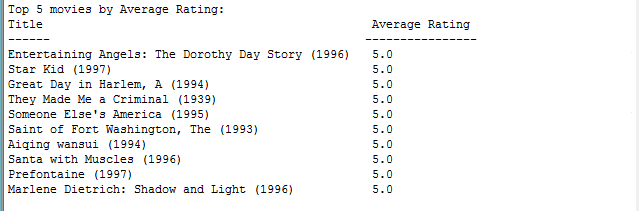
\includegraphics[width=1\textwidth]{pics/highestAverage}
\caption{Highest Average Ratings}
\label{fig:average}
\end{figure}

%%%Question 2%%%%%%%%%%%%%%%%%%%%%%%%%%%%%%%%%%%%%%%%%

\subsection{Most Ratings}
What 5 movies received the most ratings?
 Show the movies and the number of ratings sorted by number of ratings.

\subsubsection{Solution}
The same function, getRatings, was used as inthe first question.  
The data was sorted differently, on the length of the ratings list, for each movie.
Since the sorting had to be completed by the rating list length, instead of an average value , the print statements had to be written separately.
Listing \ref{code:most} is the additional code used in the getRatings function.\\

\lstset{
    caption={Get Most Ratings Code},
     label=code:most
}
\lstinputlisting[language=Python, firstline=197, lastline=207]{recommendations.py}

\subsubsection{Result}
There were no surprises to me, in this list of top rated movies, since I have seen all of them.
I did not see any ties, so for the assignment, it was not included.
Figure \ref{fig:most} shows the output.

\begin{figure}[H]
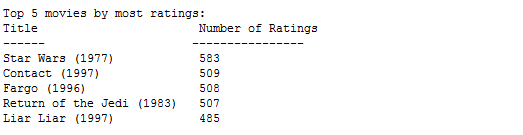
\includegraphics[width=1\textwidth]{pics/mostRatings}
\caption{Most Ratings}
\label{fig:most}
\end{figure}

%%%Question 3%%%%%%%%%%%%%%%%%%%%%%%%%%%%%%%%%%%%%%%%

\subsection{Highest Average by Women}
What 5 movies were rated the highest on average by women?
Show the movies and their ratings sorted by ratings.

\subsubsection{Solution}
A separate module was written for the gender classifications, because additional user information was needed.
Module loadUserInfo placed the user id to movie rating mappings with a nested dictionary with age and gender.\cite{bib:nested}
The loadMovieRatings module was used again, for consistency and reuse of average and printing functions.
A dictionary was created for women, initialized with each movie id.  
If a user's gender was F, for female, the movie list was checked if the user had rated it and the rating was added to the women dictionary.
Once all the women ratings were found, the average for each was calculated using ratingAverage and saved in the dictionary with movies.
In order to prevent KeyErrors, if there was a movie with no average for women, it was set to negative infinity.\cite{bib:pycookbook}
Since we were only interested in the highest ratings, it had no affect on the results.
Then the results were printed using printRatings, as shown in Listing \ref{code:highest}, for the top highest average.
Listing \ref{code:gender} is the loadUserInfo and getRatingsByGender modules.\\

\lstset{
    caption={Get Top Ratings by Gender Module},
     label=code:gender
}
\lstinputlisting[language=Python, firstline=209, lastline=270]{recommendations.py}

\subsubsection{Result}
Surprisingly, only one movie, Prefontaine (1997), was in both highest average list and the women's top ratings list.
This leads me to believe that men and women tend to disagree on movie ratings.
There were also more then five, but the output says ``Top 5'' to meet the question requirement.
Figure \ref{fig:women} shows the list.

\begin{figure}[H]
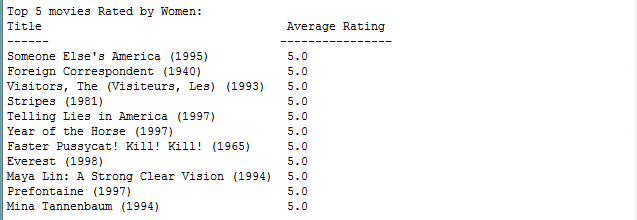
\includegraphics[width=1\textwidth]{pics/topWomen}
\caption{Highest Average Ratings by Women}
\label{fig:women}
\end{figure}

%%%Question 4%%%%%%%%%%%%%%%%%%%%%%%%%%%%%%%%%%%%%%%%%%%%

\subsection{Highest Average by Men}
What 5 movies were rated the highest on average by men? 
Show the movies and their ratings sorted by ratings.

\subsubsection{Solution}
The same module was used for men as it was for women.
A separate dictionary was created for men, to store the movie ratings and average.
If a user's gender was not F, the movie list was checked if the user had rated it and if so, the rating was added to the men dictionary.
Once all the men ratings were found, the average for each was calculated using ratingAverage and saved in the dictionary with movies.
In order to prevent KeyErrors, if no man rated a movie, it was set to negative infinity, as with the code for women.\cite{bib:pycookbook}
The code for men was included in listing \ref{code:gender}.

\subsubsection{Result}
I found that there were more top rated movies by men that matched the highest average movies from question 1.
This tells me that women must not have rated the top rated movies by men that also appear on the highest average list. 
Prefontaine (1997) was on the list for both men and women, so everyone rated that movie equally high.
Again, there were more than five, but for the purposes of the assignment, the output still states ``Top 5.''
Figure \ref{fig:men} shows the output.

\begin{figure}[H]
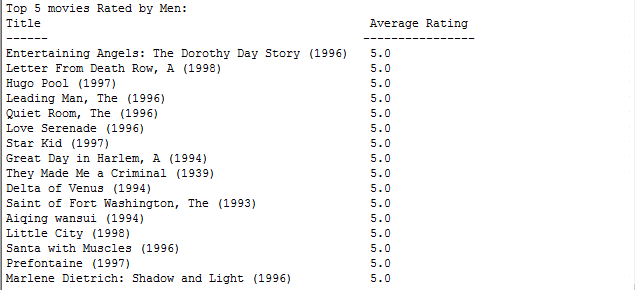
\includegraphics[width=1\textwidth]{pics/topMen}
\caption{Highest Average Ratings by Men}
\label{fig:men}
\end{figure}

%%%Question 5%%%%%%%%%%%%%%%%%%%%%%%%%%%%%%%%%%%%%%%%%%%%

\subsection{Top Gun Correlation}
What movie received ratings most like Top Gun? 
Which movie received ratings that were least like Top Gun (negative correlation)?

\subsubsection{Solution}
In order to find a movie with the closest correlation to Top Gun, calculateSimilarItems, which was included in the original code, was used. 
The original was written only for movies, so it was modified to allow for finding similar users as well.
The statement to invert the dictionary was removed and I made sure I was sending the correct dictionary to be used.
Additionally, it was set to use the sim\_pearson function, for correlation.
To get the lowest negative correlation, two additional functions were written similarly.  
The main difference was botMatches was written to return the worst correlation.
The modules for sim\_pearson was unchanged.
The loadMovie was used to retrieve with the user rating list, per movie, which is the reverse of the original loadMovieLens.
This allowed for the correlation to be calculated based on user ratings per movie.\cite{bib:collective}
Top Gun had to be found in the movie list, so the movie most similar and dissimilar could be retrieved from the results of calculateSimilarItems and calculateDissimilarItems.
Listing \ref{code:topgun} is the functions written to get the Top Gun correlation.\\

\lstset{
    caption={Top Gun Correlation Module},
     label=code:topgun
}
\lstinputlisting[language=Python, firstline=272, lastline=352]{recommendations.py}

\subsubsection{Result}
Figure \ref{fig:topgun} shows the movies with ratings most like and most unlike Top Gun.
I have not seen either of the movies in the output, so I do not have an opinion about the correlation.

\begin{figure}[H]
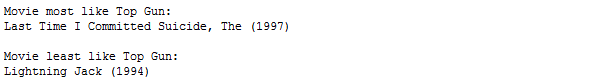
\includegraphics[width=1\textwidth]{pics/topGun}
\caption{Top Gun Correlation}
\label{fig:topgun}
\end{figure}

%%%Question 6%%%%%%%%%%%%%%%%%%%%%%%%%%%%%%%%%%%%%%%%%%%

\subsection{Top Raters}
Which 5 raters rated the most films? 
Show the raters' IDs and the number of films each rated.

\subsubsection{Solution}
A new module, loadUserRatings, was written to compile a dictionary of users with a list of their movie ratings.
Using this, the top raters were found by using the length of the list of movie ratings.
Listing \ref{code:topraters} shows the loadUserRatings and getTopRaters module.\\

\lstset{
    caption={Top Raters Module},
     label=code:topraters
}
\lstinputlisting[language=Python, firstline=354, lastline=372]{recommendations.py}

\subsubsection{Result}
There were no ties, so the top five were printed.
Figure \ref{fig:topraters} shows the user ID and number of films each rated.

\begin{figure}[H]
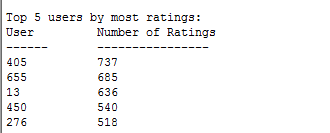
\includegraphics[width=1\textwidth]{pics/topRaters}
\caption{Top Raters}
\label{fig:topraters}
\end{figure}

%%%Question 7%%%%%%%%%%%%%%%%%%%%%%%%%%%%%%%%%%%%%%%%%%%%

\subsection{User Agreement}
Which 5 raters most agreed with each other? 
Show the raters' IDs and Pearson's r, sorted by r.

\subsubsection{Solution}
My solution used calculateSimilarItems to find the user closest to each.
For each user, a chain was created by joining the user closest to it.
Each linked userid was put into a list and the links with r and distance values were put together into a dictionary.
The list of links were converted to a set, to keep the values unique, because in testing I found some users linked back to each other, creating a loop.
At the end of the assignment I realized I could have grabbed more results and added to the chain with the next closest user, but there was not enough time to test it.
The chain was searched for the shortest distance along the chain.
Listing \ref{code:agree} is the module.\\

\lstset{
    caption={},
     label=code:agree
}
\lstinputlisting[language=Python, firstline=374, lastline=410]{recommendations.py}

\subsubsection{Result}
I would think that if two users had ratings close to each other, the r value would be positively correlated.
My results did not support this, the Pearson value was calculated to be zero.
When testing, this intuition seemed to be correct for chains up to four.
This leads me to believe that my algorithm for finding the five closest was not correct.
Figure \ref{fig:agree} shows the result.

\begin{figure}[H]
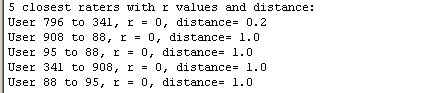
\includegraphics[width=1\textwidth]{pics/agree}
\caption{User Agreement}
\label{fig:agree}
\end{figure}

%%%Question 8%%%%%
\subsection{User Disagreement}
Which 5 raters most disagreed with each other (negative correlation)? 
Show the raters' IDs and Pearson's r, sorted by r.

\subsubsection{Solution}
The code to find the 5 raters who disagreed was the same as the code for agreement, except using calcuateDissimilarItems.
Listing \ref{code:disagree} is the additional code in getUserCorrelation.\\

\lstset{
    caption={User Disagreement},
     label=code:disagree
}
\lstinputlisting[language=Python, firstline=411, lastline=443]{recommendations.py}

\subsubsection{Result}
My results for disagreement also do not follow what I would expect.
All of the Pearson r values were zero, whereas I would expect them to be negative.
Figure \ref{fig:disree} shows the result.

\begin{figure}[H]
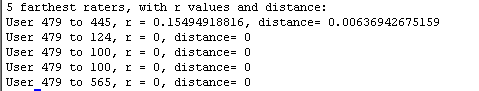
\includegraphics[width=1\textwidth]{pics/disagree}
\caption{User Disagreement}
\label{fig:disagree}
\end{figure}

%%%Question 9%%%%%
\subsection{Men by Age}
What movie was rated highest on average by men over 40? 
By men under 40?

\subsubsection{Solution}
This solution was similar to the gender based solution. 
The modules used to import the data were loadMovieRatings from listing \ref{code:highest} and loadUserInfo from listing \ref{code:gender}.
Dictionaries were created for both gender based age groups, so the averages could be calculated independently.
Then for each user, gender and age were checked, and the rating for each movie was added.
Next the averages were calculated using ratingAverage, as in listing \ref{code:highest}.
If the movie was not rated by that group, it was set to negative infinity, since it would not affect the highest average outcome.
Then the results were printed using printRatings, also from listing \ref{code:highest}.
Listing \ref{code:age} is the function getRatingsByAge.\\

\lstset{
    caption={Ratings by Age},
     label=code:age
}
\lstinputlisting[language=Python, firstline=446, lastline=522]{recommendations.py}

\subsubsection{Result}
Althought the requirement was for five, there were more that had a average rating of 5.0.
There were a few movies from the top rated men's list that were also on the list for men over 40.
Figure \ref{fig:mO40} shows the list.
However, most of the movies on the men under 40 list, as shown in Figure \ref{fig:mU40}, were also on the top rated men's list.
This tells me that most of the movies on the top rated men's list were not rated by men over 40.
The movie Prefontaine (1997) was on both lists, so again, it was liked by everyone.

\begin{figure}[H]
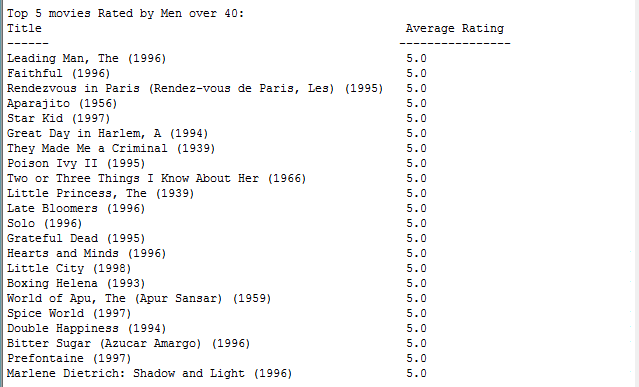
\includegraphics[width=1\textwidth]{pics/topMenO40}
\caption{Top Ratings Men over 40}
\label{fig:mO40}
\end{figure}

\begin{figure}[H]
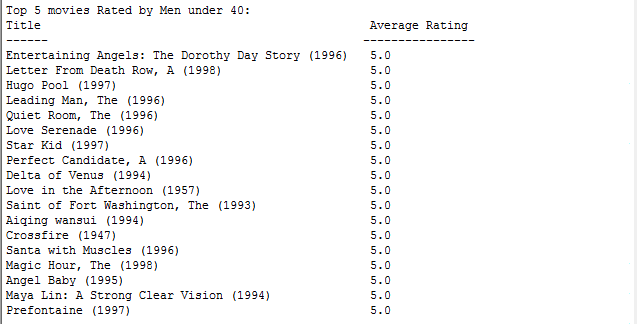
\includegraphics[width=1\textwidth]{pics/topMenU40}
\caption{Top Ratings Men under 40}
\label{fig:mU40}
\end{figure}

%%%Question 10%%%%%
\subsection{}
What movie was rated highest on average by women over 40?
 By women under 40?

\subsubsection{Solution}
The solution for getting the ratings for women by age group was also in getRatingsByAge, shown in listing \ref{code:age}.
Again, separate dictionaries were created to consolidate ratings and calculate the averages independently.

\subsubsection{Result}
There were few movies in the women over 40 group that were also in the women's top rated list.
This was the first list that did not include the movie  Prefontaine (1997), so women over 40 must not watch this movie.
Figure \ref{wO40} shows the list.
As with the men, most of the movies in the women under 40 group were in the women's top rated list, shown in Figure \ref{wU40}.
 Prefontaine (1997) was also in the list, as it was in both groups of men.

\begin{figure}[H]
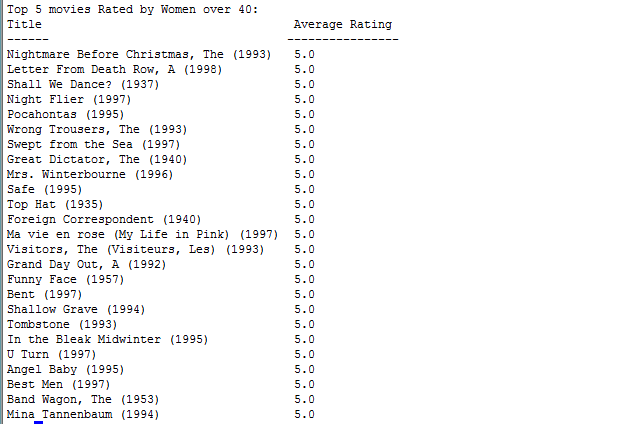
\includegraphics[width=1\textwidth]{pics/topWomenO40}
\caption{Top Ratings Women over 40}
\label{fig:wO40}
\end{figure}

\begin{figure}[H]
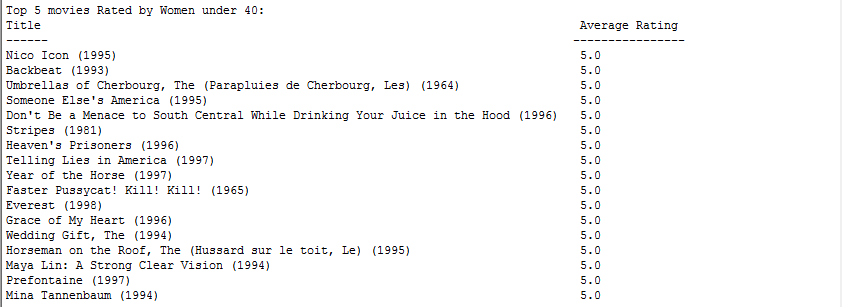
\includegraphics[width=1.2\textwidth]{pics/topWomenU40}
\caption{Top Ratings Women under 40}
\label{fig:wU40}
\end{figure}

\newpage
\subsection{Python Code}
\label{sec:rec-code}
%%% Code Listing%%%%%

\lstset{
    language=python,
    caption={Python Recommendations},
     label=code:recommendations
}

\lstinputlisting{recommendations.py}
\newpage 


\bibliography{references}{}
\bibliographystyle{plain}
\end{document}